\chapter{Search for semi-visible jets}  % might want to be more specific with the title if it only considers the generator-level studies
\label{chap:svj}

\epigraph{Of darkness visible so much be lent, as half to show, half veil, the deep intent.}{--- Alexander Pope}

\initial{T}his is the analysis chapter on \glspl{svj}.

%=======
\begin{easylist}[itemize]
    \easylistprops
    & Not 100\% sure whether this should go between theory and detector chapters, between detector and objects, or between objects and Hinv.
    && This could even be appended onto to the SVJ bit in the theory chapter, instead. Though, there would be a reasonable amount of material and discussion, so probably deserves its own (short) chapter
    & Only really discuss my contributions: $s$- and \tchannel signal model production and understanding. Can go into reasonable detail -- at the level of the AN or perhaps deeper
    && Show \schannel comparisons between \MADGRAPH and \PYTHIA, as shown in the AN, and discuss merits of using either method (easier to specify in \PYTHIA and matrix element calculations should be equivalent to \MADGRAPH, but latter is required for \tchannel and makes sense to have consistency)
    && Show a few distributions from \tchannel signal, just for some insight as to how they differ from \schannel. Not sure if they need some sort of approval since they're generated with \acrshort{cmssw}
    && Note that these are before any cuts, so comparing right what comes out of the generator + \acrshort{cmssw} processing pipeline. Could even potentially make some plots after applying analysis preselection that could clean up some events
    && Objects (AK4 jets, AK8 jets, MET) are straight out of nanoAOD, without the further processing and quality cuts that go into the Hinv objects. Though, since the objects have gone through the full CMSSW processing pipeline, there should be at least some intrinsic level of quality of the objects.
    && Note that we use SVJ\_3000\_20\_0.3\_peak in the analysis as benchmark point (see AN for \emph{why}). Theorists use 1000\_10 (rinv ?, alpha\_d ?). Tending to vary points around that. Note the convention for labelling the mass points: SVJ\_$\expval{m_{\mathrm{mediator}}}$\_$\expval{\mDark}$\_$\expval{\rinv}$\_$\expval{\aDark}$.
    && Also say that my \MADGRAPH implementation has been built upon for the upcoming \tchannel and boosted \PZprime searches
    & Perhaps give a brief summary of the analysis: dijet search, using an SVJ tagger, transverse mass as fit variable. Say that details/complete description is discussed in the paper/Giorgia's thesis (with references)
\end{easylist}

% Can pull from Section 35 of my lab book, and all the talks I and other people from the team have given (Presentations and talks/ folder, also Other peoples/ subdirectory). Can also pull from AN for theory, translation of some theory stuff into experiment, and analysis strategy


%=========================================================


\section{Analysis summary}
\label{sec:svj_overview}


%=========================================================


\section{Data and simulation}
\label{sec:svj_data_sim}

In the main analysis for the \schannel signal model, \PYTHIA is used as it can parametrise all the relevant aspects of the model in a simple manner with high efficiency. \MADGRAPH is the often-preferred generator as it can handle more complex models and decays. For the \schannel mode, the scattering matrix element calculations that model the hard process are identical between \PYTHIA and \MADGRAPH. In the former, the characterisation, interactions, and decays of the dark sector particles are implemented via the \texttt{Hidden Valley} module, available from \PYTHIA~8.226. Samples generated with \MADGRAPH are hadronised by \PYTHIA as part of the full simulation chain within \acrshort{cmssw}. \Gls{jet} matching and filter efficiencies may noticeably reduce the final number of events . The \tchannel model is possible to parametrise in \PYTHIA, but due to its complexity, we opt to do so in \MADGRAPH. Hadronisation, however, is still performed by \PYTHIA. % large number of subprocesses and potential diagrams in t-channel

The full description of \schannel signal generation with \PYTHIAEIGHT is given in Chpt.~\ref{subsec:svj_signal_pythia}. An equivalent implementation where the hard scatter is modelled in \MGvATNLO, as both an alternative and cross-check to the \PYTHIA [version], is [described] in Chpt.~\ref{subsec:svj_signal_madgraph}. A description of the \tchannel process is also present. Comparisons between the \PYTHIA and \MADGRAPH implementations are [given] in Chpt.{}


%=========================================================


\subsection{Generating signal samples in \texorpdfstring{\PYTHIA}{Pythia}}
\label{subsec:svj_signal_pythia}

The \texttt{Hidden Valley} module allows for $\HepProcess{\Pquark\APquark \to \PZprime \to \Pqdark\Paqdark}$, where $\PZprime$ is acts as intended as a portal between the visible and dark sectors. Since we expect a small percentage of them to decay visibly, a branching ratio to each of the six \acrshort{sm} quarks is set to 0.003. The remaining fraction of 0.982 decays to $\Pqdark\Paqdark$, where $\Pqdark$ is a Hidden Valley particle charged only under that gauge group. Dark quarks hadronise into one of two types of dark meson that correspond to particles from the \texttt{Hidden Valley} module: \Ppidark and \Prhodark, that are pseudoscalar and vector, respectively. Each possess flavour-diagonal and off-diagonal variants. They are set to decay invisibly with a branching fraction \rinv. Remaining decay modes may be either democratic (equal probability) to \acrshort{sm} quark-antiquark pairs,\footnote{Top quarks are excluded in all cases, since in the scan of model parameters where we predict the greatest sensitivity, the dark mesons are always too light to decay on shell to a \ttbar pair.} or by accounting for running quark masses.\footnote{Will have to explain running masses/mass insertion later on.}

% Describe Z2 and dark quark filters as well
% Look in AN for more description regarding the dark hadrons, decays of dark mesons, etc.


%=========================================================


\subsection{Generating signal samples in \texorpdfstring{\MADGRAPH}{MadGraph}}
\label{subsec:svj_signal_madgraph}

% Generating s-channel samples from my repo should be pretty consistent with Kevin's

% Able to generate s- and t-channel signal in MadGraph and Pythia for 2016, 17 and 18. Important since it's a full Run-2 analysis

% Add t-channel plots as well, potentially with s-channel overlaid to show how different signals are

% Mention something about matching efficiency decreases as r_inv increases (since more of the event is invisible, fewer jets pass the qCut - also explain exactly what qCut is)


%=========================================================


\subsubsection{\texorpdfstring{\schannel}{s-channel}}
\label{subsubsec:svj_signal_madgraph_schannel}

% Might not be any point showing only s-channel MadGraph signal since the curves are given in the comparison plots. Though, I could instead showcase some plots from the benchmark mass point, and variations around that (e.g., vary mZp up and down by a factor of 2, then same with m_dq, r_inv, and then alpha_d_low and alpha_d_high)


%=========================================================


\subsubsection{\texorpdfstring{\tchannel}{t-channel}}
\label{subsubsec:svj_signal_madgraph_tchannel}

% Will have to decide whether to show s-channel and t-channel on same axes, or separately


%=========================================================


\subsection{\texorpdfstring{\PYTHIA}{Pythia}-\texorpdfstring{\MADGRAPH}{MadGraph} comparisons for \texorpdfstring{\schannel}{s-channel} signal}
\label{subsec:svj_schannel_comparisons}

% A "jet" here is a AK8 jet

\begin{figure}[htbp]
    \centering
    \begin{subfigure}[b]{0.45\textwidth}
        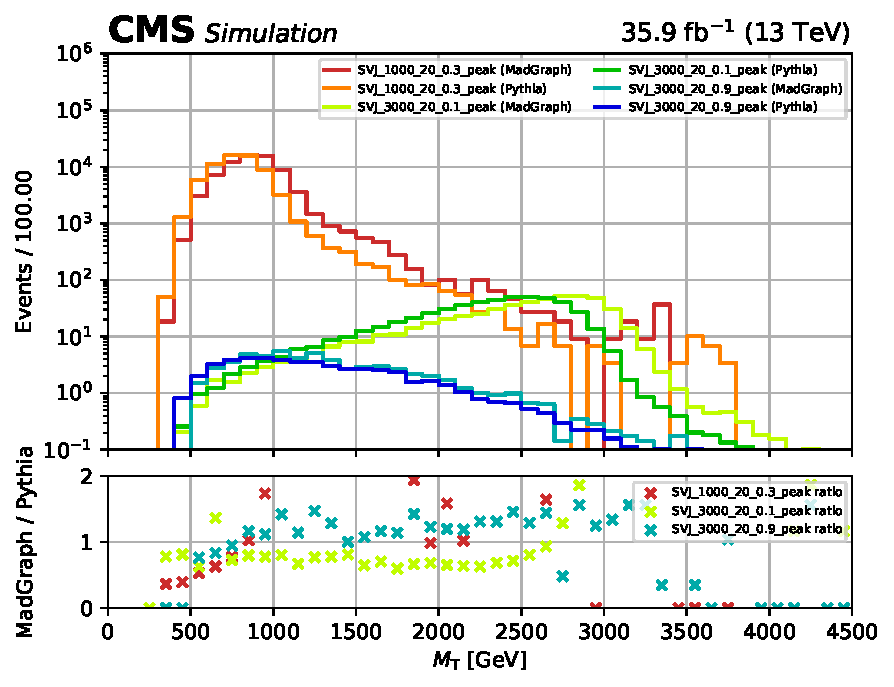
\includegraphics[width=\textwidth]{figures/madgraph_pythia_comparisons/with_ratios/part1/dijet_mt.pdf}
        \caption{Transverse mass of the dijet system}
    \end{subfigure}
    \hfill
    \begin{subfigure}[b]{0.45\textwidth}
        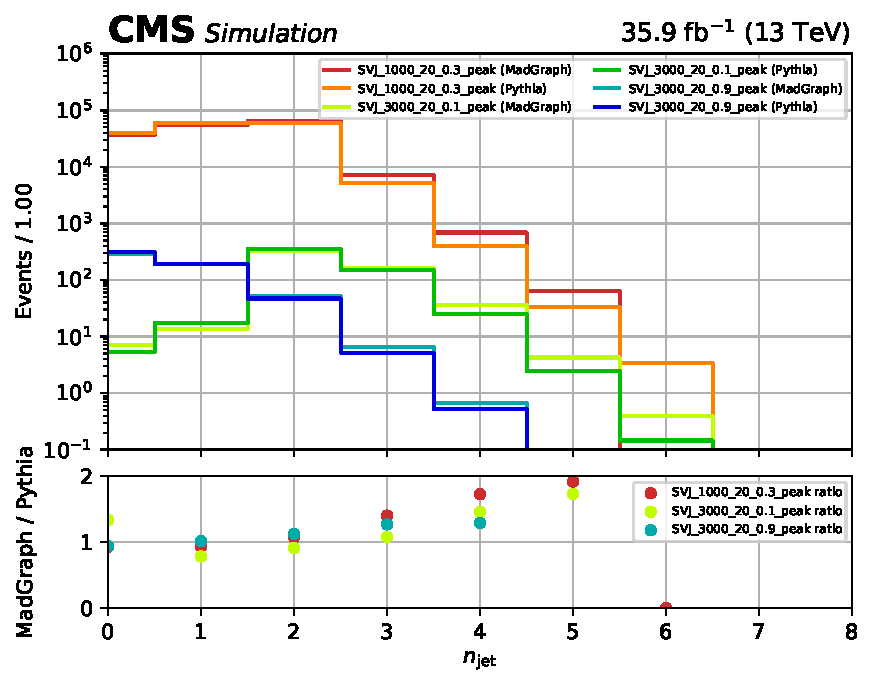
\includegraphics[width=\textwidth]{figures/madgraph_pythia_comparisons/with_ratios/part1/njet.pdf}
        \caption{\njet}
    \end{subfigure}

    \begin{subfigure}[b]{0.45\textwidth}
        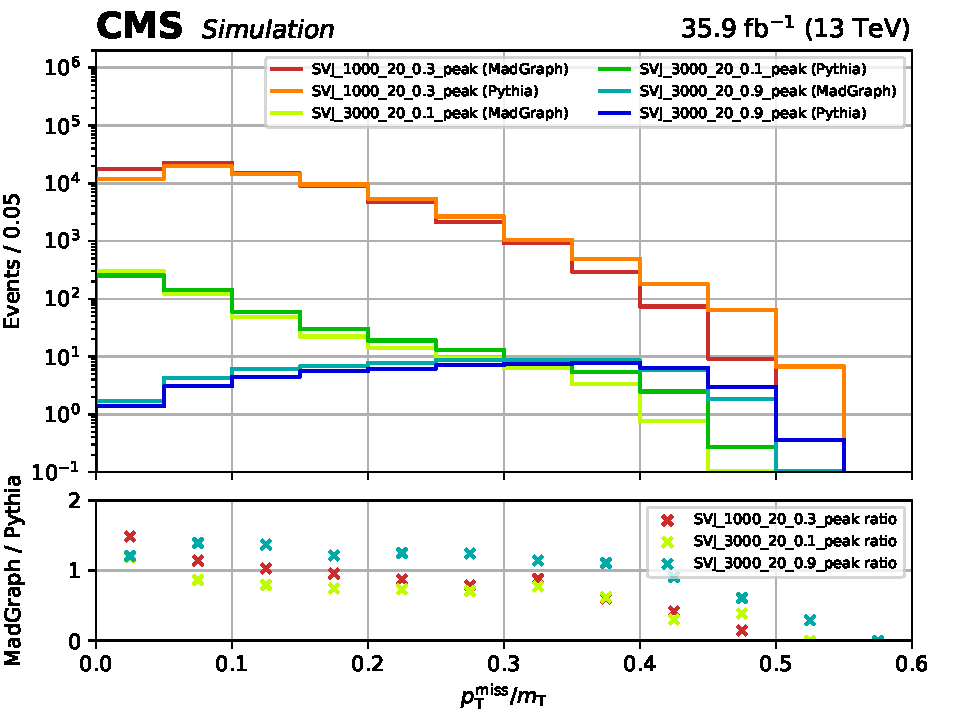
\includegraphics[width=\textwidth]{figures/madgraph_pythia_comparisons/with_ratios/part1/met_over_mt.pdf}
        \caption{$\MET/\mT$}
    \end{subfigure}
    \hfill
    \begin{subfigure}[b]{0.45\textwidth}
        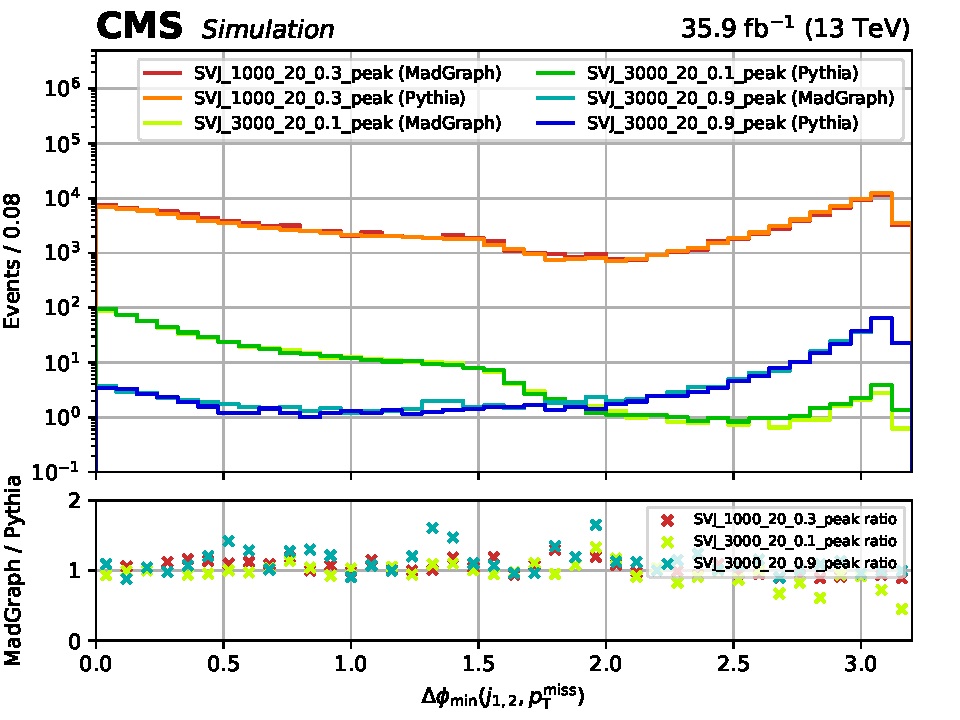
\includegraphics[width=\textwidth]{figures/madgraph_pythia_comparisons/with_ratios/part1/min_dphi.pdf}
        \caption{\mindphi between \MET and two leading \glspl{jet}}
    \end{subfigure}
    \caption[Distributions of several observables for the models SVJ\_1000\_20\_0.3\_peak, SVJ\_3000\_20\_0.1\_peak, and SVJ\_3000\_20\_0.9\_peak]{Distributions of several observables for the models SVJ\_1000\_20\_0.3\_peak, SVJ\_3000\_20\_0.1\_peak, and SVJ\_3000\_20\_0.9\_peak. Generation in \MGvATNLO is compared to \PYTHIAEIGHT, with the ratios between them for each model displayed in the respective subplot.}
    \label{fig:svj_mg_pythia_comparison_set1}
\end{figure}

\begin{figure}[htbp]
    \centering
    \begin{subfigure}[b]{0.45\textwidth}
        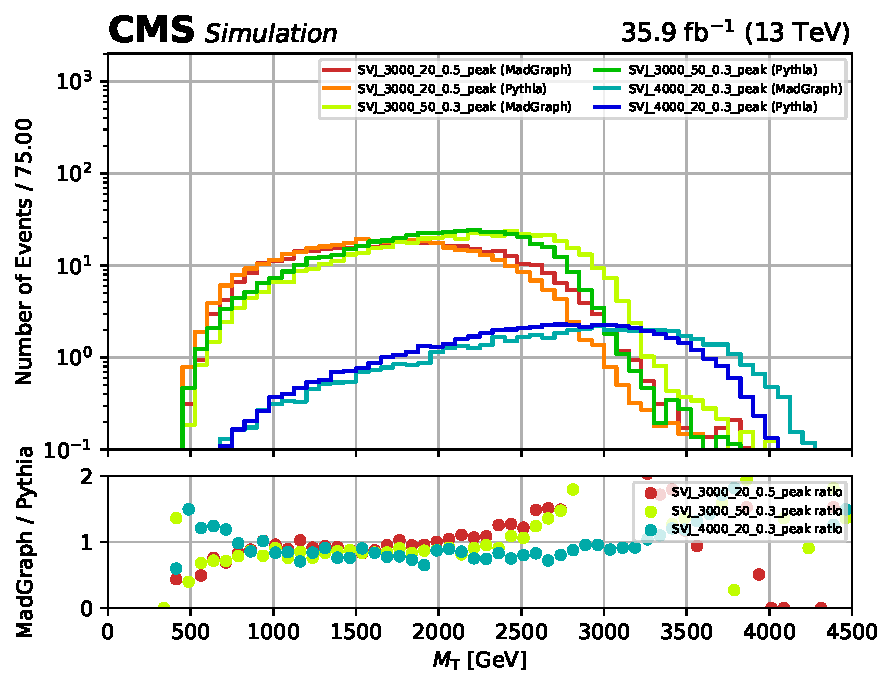
\includegraphics[width=\textwidth]{figures/madgraph_pythia_comparisons/with_ratios/part2/dijet_mt.pdf}
        \caption{Transverse mass of the dijet system}
    \end{subfigure}
    \hfill
    \begin{subfigure}[b]{0.45\textwidth}
        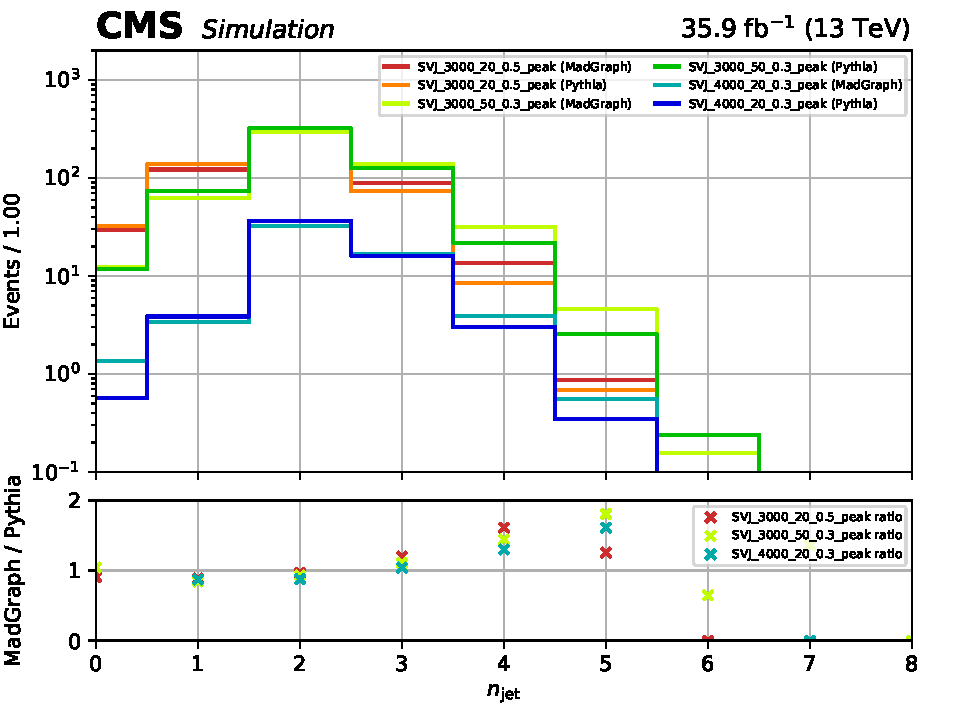
\includegraphics[width=\textwidth]{figures/madgraph_pythia_comparisons/with_ratios/part2/njet.pdf}
        \caption{\njet}
    \end{subfigure}

    \begin{subfigure}[b]{0.45\textwidth}
        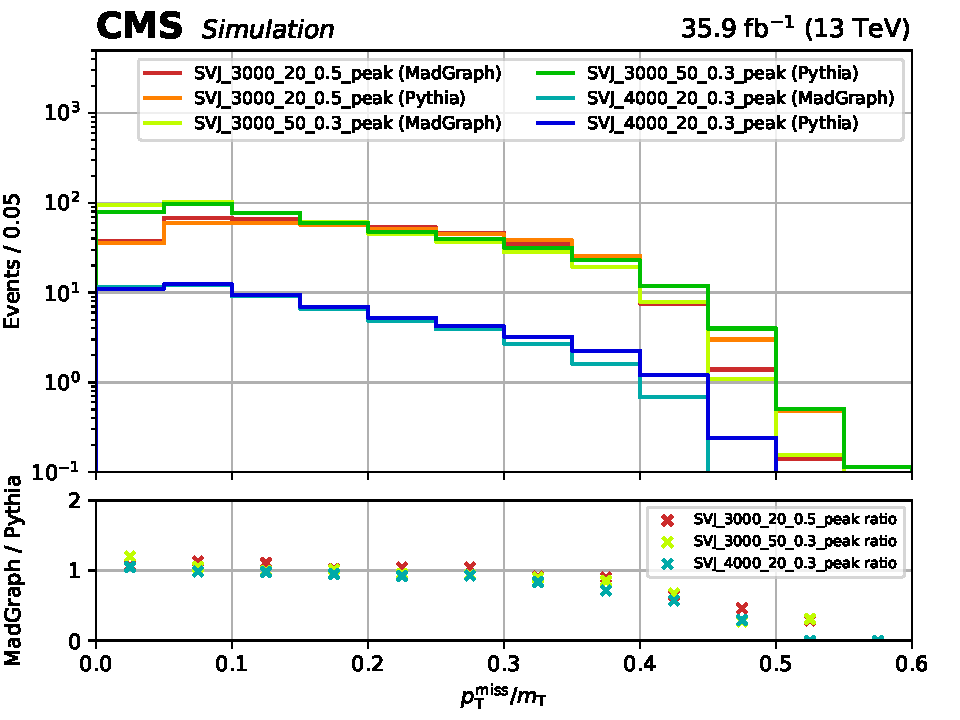
\includegraphics[width=\textwidth]{figures/madgraph_pythia_comparisons/with_ratios/part2/met_over_mt.pdf}
        \caption{$\MET/\mT$}
    \end{subfigure}
    \hfill
    \begin{subfigure}[b]{0.45\textwidth}
        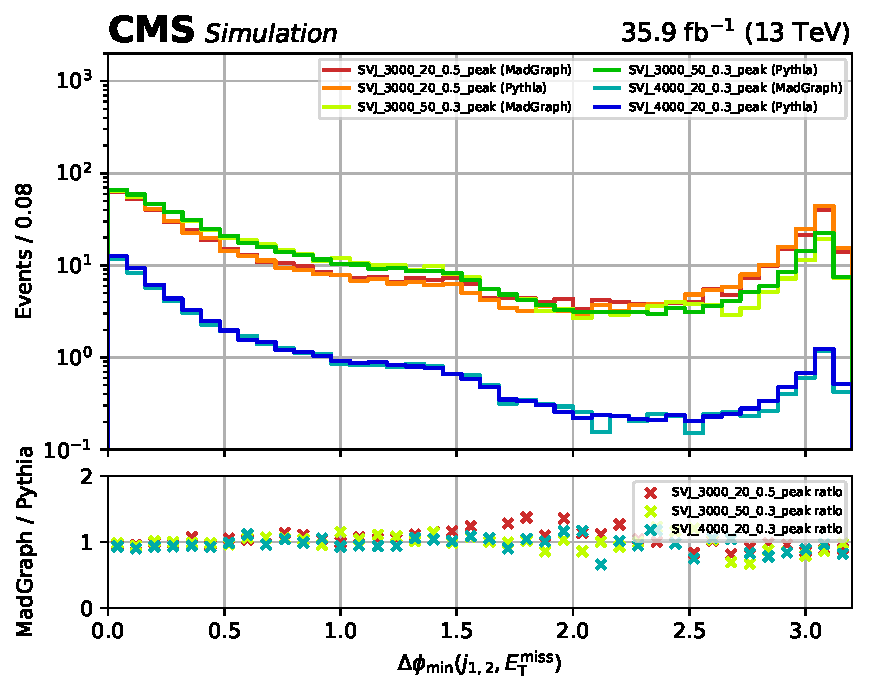
\includegraphics[width=\textwidth]{figures/madgraph_pythia_comparisons/with_ratios/part2/min_dphi.pdf}
        \caption{\mindphi between \MET and two leading \glspl{jet}}
    \end{subfigure}
    \caption[Distributions of several observables for the models SVJ\_3000\_20\_0.5\_peak, SVJ\_3000\_50\_0.3\_peak, and SVJ\_4000\_20\_0.3\_peak]{Distributions of several observables for the models SVJ\_3000\_20\_0.5\_peak, SVJ\_3000\_50\_0.3\_peak, and SVJ\_4000\_20\_0.3\_peak. Generation in \MGvATNLO is compared to \PYTHIAEIGHT, with the ratios between them for each model displayed in the respective subplot.}
    \label{fig:svj_mg_pythia_comparison_set2}
\end{figure}
